\subsection{Exercise 28.4}

\noindent \hspace{1.2em}\textit{Find the volume of the solid of revolution formed by rotating the regions bounded by the following curves and lines about the $x$-axis (Question 1 to 7):}

\begin{enumerate}
      \begin{multicols}{2}
            \item $y=\sqrt{x}, x=4, x=9$, and $x$-axis
            \sol{}
            \begin{flalign*}
                  V_x & = \int_{4}^{9} \pi \left( \sqrt{x} \right)^2 dx & \\
                      & = \pi \int_{4}^{9} x dx                         & \\
                      & = \pi \left[ \frac{x^2}{2} \right]_{4}^{9}      & \\
                      & = \pi \left( \frac{81}{2} - 8 \right)           & \\
                      & = \frac{65 \pi}{2}
            \end{flalign*}

            \item $y=3 x, x=4$, and $x$-axis
            \sol{}
            \begin{flalign*}
                  V_x & = \int_{0}^{4} \pi \left( 3 x \right)^2 dx & \\
                      & = \pi \int_{0}^{4} 9 x^2 dx                & \\
                      & = \pi \left[ 3 x^3 \right]_{0}^{4}         & \\
                      & = 192 \pi
            \end{flalign*}
      \end{multicols}

      \begin{multicols}{2}
            \item $y=x(x-2)$, and $x$-axis
            \sol{}
            \begin{flalign*}
                  V_x & = \pi \int_{0}^{2} x^2 (x-2)^2 dx                                 & \\
                      & = \pi \int_{0}^{2} x^2 (x^2 - 4x + 4) dx                          & \\
                      & = \pi \int_{0}^{2} x^4 - 4x^3 + 4x^2 dx                           & \\
                      & = \pi \left[ \frac{x^5}{5} - x^4 + \frac{4x^3}{3} \right]_{0}^{2} & \\
                      & = \pi\left[\dfrac{32}{5} - 16 + \dfrac{32}{3}\right]              & \\
                      & = \dfrac{16 \pi}{15}
            \end{flalign*}

            \item $x^2+y^2=4, x=0$, and $x=2$
            \sol{}
            \begin{flalign*}
                  V_x & = \pi \int_{0}^{2} \left( 4 - x^2 \right) dx    & \\
                      & = \pi \left[ 4x - \frac{x^3}{3} \right]_{0}^{2} & \\
                      & = \frac{16 \pi}{3}
            \end{flalign*}
      \end{multicols}

      \begin{multicols}{2}
            \item $y=\sin x, x=0, x=\pi$, and $x$-axis
            \sol{}
            \begin{flalign*}
                  V_x & = \pi \int_{0}^{\pi} \sin^2 x dx                               & \\
                      & = \pi \int_{0}^{\pi} \frac{1 - \cos 2x}{2} dx                  & \\
                      & = \frac{\pi}{2} \int_{0}^{\pi} (1 - \cos 2x) dx                & \\
                      & = \frac{\pi}{2} \left[ x - \frac{\sin 2x}{2} \right]_{0}^{\pi} & \\
                      & = \frac{\pi}{2} \left( \pi - 0 \right)                         & \\
                      & = \frac{\pi^2}{2}
            \end{flalign*}

            \item $y=e^x, x=-1, x=1$, and $x$-axis
            \sol{}
            \begin{flalign*}
                  V_x & = \pi \int_{-1}^{1} e^{2x} dx                         & \\
                      & = \pi \left[ \frac{e^{2x}}{2} \right]_{-1}^{1}        & \\
                      & = \pi \left( \frac{e^2}{2} - \frac{e^{-2}}{2} \right) & \\
                      & = \frac{\pi}{2} \left( e^2 - e^{-2} \right)
            \end{flalign*}
      \end{multicols}

      \newpage
      \item $y=x^3+x^2-2 x$, and $x$-axis
            \sol{}
            \begin{flalign*}
                  V_x & = \pi \int_{-2}^{1} \left( x^3 + x^2 - 2 x \right)^2 dx                                                                                                  & \\
                      & = \pi \int_{-2}^{1} (x^6 + x^4 + 4x^2 + 2x^5 - 4x^3 - 4x^4) dx                                                                                           & \\
                      & = \pi \int_{-2}^{1} (x^6 + 2x^5 - 3x^4 - 4x^3 + 4x^2) dx                                                                                                 & \\
                      & = \pi \left[ \frac{x^7}{7} + \frac{x^6}{3} - \dfrac{3}{5}x^5 - x^4 + \frac{4x^3}{3} \right]_{-2}^{1}                                                     & \\
                      & = \pi \left( \dfrac{1}{7} + \dfrac{1}{3} - \dfrac{3}{5} - 1 + \dfrac{4}{3} + \dfrac{128}{7} - \dfrac{64}{3} - \dfrac{96}{5} + 16 + \dfrac{32}{3} \right) & \\
                      & = \dfrac{162}{35} \pi
            \end{flalign*}
\end{enumerate}

\noindent \hspace{1.2em}\textit{Find the volume of the solid of revolution formed by rotating the regions bounded by the following curves and lines about the $y$-axis (Question 8 to 14):}

\begin{enumerate}[resume]
      \begin{multicols}{2}
            \item $y=x^3, y=8$, and $y$-axis
            \sol{}
            \begin{flalign*}
                  V_y & = \pi \int_{0}^{8} \left( \sqrt[3]{y} \right)^2 dy       & \\
                      & = \pi \int_{0}^{8} y^{\frac{2}{3}} dy                    & \\
                      & = \pi \left[ \frac{3}{5} y^{\frac{5}{3}} \right]_{0}^{8} & \\
                      & = \frac{3 \pi}{5} \left( 8^{\frac{5}{3}} - 0 \right)     & \\
                      & = \frac{96 \pi}{5}
            \end{flalign*}

            \item $x=\sqrt{y-1}, y=4$, and $y$-axis
            \sol{}
            \begin{flalign*}
                  V_y & = \pi \int_{1}^{4} \left( \sqrt{y-1} \right)^2 dy & \\
                      & = \pi \int_{1}^{4} (y-1) dy                       & \\
                      & = \pi \left[ \frac{y^2}{2} - y \right]_{1}^{4}    & \\
                      & = \pi \left( 8 - 4 - \frac{1}{2} + 1 \right)      & \\
                      & = \frac{9 \pi}{2}
            \end{flalign*}
      \end{multicols}

      \begin{multicols}{2}
            \item $y^2=x+3, y=2, x$-axis, and $y$-axis
            \sol{}
            \begin{flalign*}
                  V_y & = \pi \int_{0}^{2} \left( y^2 - 3 \right)^2 dy           & \\
                      & = \pi \int_{0}^{2} (y^4 - 6 y^2 + 9) dy                  & \\
                      & = \pi \left[ \frac{y^5}{5} - 2 y^3 + 9 y \right]_{0}^{2} & \\
                      & = \pi \left( \frac{32}{5} - 16 + 18 \right)              & \\
                      & = \frac{42 \pi}{5}
            \end{flalign*}

            \item $y^2=x+1$, and $y$-axis
            \sol{}
            \begin{flalign*}
                  V_y & = \pi \int_{-1}^{1} \left( y^2 - 1 \right)^2 dy                                    & \\
                      & = \pi \int_{-1}^{1} (y^4 - 2 y^2 + 1) dy                                           & \\
                      & = \pi \left[ \frac{y^5}{5} - \frac{2 y^3}{3} + y \right]_{-1}^{1}                  & \\
                      & = \pi \left( \frac{1}{5} - \frac{2}{3} + 1 + \frac{1}{5} - \frac{2}{3} + 1 \right) & \\
                      & = \frac{16 \pi}{15}
            \end{flalign*}
      \end{multicols}

      \newpage
      \begin{multicols}{2}
            \item $x^2-y^2=4, y=3$, and $x$-axis
            \sol{}
            \begin{flalign*}
                  V_x & = \pi \int_{0}^{3} (4+y^2) dy                   & \\
                      & = \pi \left[ 4y + \frac{y^3}{3} \right]_{0}^{3} & \\
                      & = \pi \left( 12 + 9 \right)                     & \\
                      & = 21 \pi
            \end{flalign*}

            \item $y=1-\sqrt{x}, x$-axis, and $y$-axis
            \sol{}
            \begin{flalign*}
                  V_x & = \pi \int_{0}^{1} \left( 1 - y \right)^4 dy                       & \\
                      & = \pi \int_{0}^{1} (1 - 4y + 6y^2 - 4y^3 + y^4) dy                 & \\
                      & = \pi \left[ y - 2y^2 + 2y^3 - y^4 + \frac{y^5}{5} \right]_{0}^{1} & \\
                      & = \pi \left( 1 - 2 + 2 - 1 + \frac{1}{5} \right)                   & \\
                      & = \frac{\pi}{5}
            \end{flalign*}
      \end{multicols}

      \item $y=\dfrac{1}{x}-1, y=1, x$-axis, and $y$-axis
            \sol{}
            \begin{flalign*}
                  V_x & = \pi \int_{0}^{1} \frac{1}{(y + 1)^2} dy
            \end{flalign*}
            Let $u = y + 1$, then $du = dy$. When $y = 0$, $u = 1$, when $y = 1$, $u = 2$.
            \begin{flalign*}
                  V_x & = \pi \int_{1}^{2} \frac{1}{u^2} du       & \\
                      & = \pi \left[ -\frac{1}{u} \right]_{1}^{2} & \\
                      & = \pi \left( -\frac{1}{2} + 1 \right)     & \\
                      & = \frac{\pi}{2}
            \end{flalign*}

      \item Given that a region is bounded by the curve $y=4-x^2$ and the $x$-axis. Find
            the volume of the solid of revolution formed by rotating this region about the
            $x$-axis and the $y$-axis respectively. \sol{}
            \begin{flalign*}
                  V_x & = \pi \int_{-2}^{2} (4-x^2)^2 dx                                                         & \\
                      & = \pi \int_{-2}^{2} (16 - 8x^2 + x^4) dx                                                 & \\
                      & = \pi \left[ 16x - \frac{8x^3}{3} + \frac{x^5}{5} \right]_{-2}^{2}                       & \\
                      & = \pi \left( 32 - \frac{64}{3} + \frac{32}{5} + 32 - \frac{64}{3} + \frac{32}{5} \right) & \\
                      & = \frac{512 \pi}{15}
            \end{flalign*}
            \begin{flalign*}
                  V_y & = \pi \int_{0}^{4} \left( 4 - y \right)dy       & \\
                      & = \pi \left[ 4y - \frac{y^2}{2} \right]_{0}^{4} & \\
                      & = \pi \left( 16 - 8 \right)                     & \\
                      & = 8 \pi
            \end{flalign*}

      \item Given that a region is bounded by the curve $y=5-\sqrt{x}, x$-axis, and
            $y$-axis. Find the volume of the solid of revolution formed by rotating this
            region about the $x$-axis and the $y$-axis respectively. \sol{} \vspace{-0.8cm}
            \begin{multicols}{2}
                  \begin{flalign*}
                        V_x & = \pi \int_{0}^{25} \left( 5 - \sqrt{x} \right)^2 dx                            & \\
                            & = \pi \int_{0}^{25} \left(25 - 10 \sqrt{x} + x\right) dx                        & \\
                            & = \pi \left[ 25x - \frac{20x^{\frac{3}{2}}}{3} + \frac{x^2}{2} \right]_{0}^{25} & \\
                            & = \pi \left( 625 - \frac{2500}{3} + \frac{625}{2} \right)                       & \\
                            & = \frac{625 \pi}{6}
                  \end{flalign*}
                  \vfill\null
                  \begin{flalign*}
                        V_y & = \pi \int_{0}^{5} \left( 5 - y \right)^4 dy                              & \\
                            & = \pi \int_{0}^{5} (y^4 - 20y^3 + 150y^2 - 500y + 625) dy                 & \\
                            & = \pi \left[ \frac{y^5}{5} - 5y^4 + 50y^3 - 250y^2 + 625y \right]_{0}^{5} & \\
                            & = \pi \left( 625 - 3125 + 6250 - 6250 + 3125 \right)                      & \\
                            & = 625 \pi
                  \end{flalign*}
                  \vfill\null
            \end{multicols}
            \vfill\null

      \item Find the volume of the solid of revolution formed by rotating the region
            bounded by the cu rve $y^2=9 x$, the line $y=6$, and the $y$-axis about the the
            $y$-axis. \sol{}
            \begin{flalign*}
                  V_y & = \pi \int_{0}^{6} \left( \frac{y^2}{9} \right)^2 dy & \\
                      & = \pi \int_{0}^{6} \frac{y^4}{81} dy                 & \\
                      & = \pi \left[ \frac{y^5}{405} \right]_{0}^{6}         & \\
                      & = \frac{7776 \pi}{405}                               & \\
                      & = \frac{96 \pi}{5}
            \end{flalign*}
            \vfill\null

      \item Given that a region is bounded by the curve $y=x^2+1$, the line $x=-2, x=2$,
            and $x$-axis. Find the volume of the solid of revolution formed by rotating
            this region about the $x$-axis and the $y$-axis respectively. \vspace{-0.8cm}
            \begin{multicols}{2}
                  \begin{flalign*}
                        V_x & = \pi \int_{-2}^{2} \left( x^2 + 1 \right)^2 dx                                                              & \\
                            & = \pi \int_{-2}^{2} (x^4 + 2x^2 + 1) dx                                                                      & \\
                            & = \pi \left[ \frac{x^5}{5} + \frac{2x^3}{3} + x \right]_{-2}^{2}                                             & \\
                            & = \pi \left( \frac{32}{5} + \frac{16}{3} + 2 + \frac{32}{5} + \frac{16}{3} + 2 \right)  = \frac{412 \pi}{15}
                  \end{flalign*}
                  \vfill\null
                  \begin{flalign*}
                        V_y & = \pi \int_{1}^{5} (y-1) dy + \pi(2)^2\cdot 1                   & \\
                            & = \pi \left[ \frac{y^2}{2} - y \right]_{1}^{5} + 4\pi           & \\
                            & = \pi \left( \frac{25}{2} - 5 - \dfrac{1}{2} + 1\right)  + 4\pi & \\
                            & = 12 \pi
                  \end{flalign*}
                  \vfill\null
            \end{multicols}
            \vfill\null

            \newpage
            \begin{multicols}{2}
                  \item Find the volume of the solid of revolution formed by \\rotating the region
                  bounded by the curve $y=x(6-x)$ \\and the line $y=3 x$ about the $x$-axis.
                  \sol{}
                  \begin{flalign*}
                        V_x & = \pi \int_{0}^{3} \left[x^2(6-x)^2 - (3x)^2\right] dx   & \\
                            & = \pi \int_{0}^{3} (x^4 - 12x^3 + 36x^2 - 9x^2) dx       & \\
                            & = \pi \int_{0}^{3} (x^4 - 12x^3 + 27x^2) dx              & \\
                            & = \pi \left[ \frac{x^5}{5} - 3x^4 + 9x^3 \right]_{0}^{3} & \\
                            & = \pi \left( \frac{243}{5} - 81 + 81 \right)             & \\
                            & = \frac{162 \pi}{5}
                  \end{flalign*}

                  \item Find the volume of the solid of revolution formed by rotating the region
                  bounded by the curve $y=x^2$, the lines $x=1$ and $y=9$ about the $y$-axis.
                  \sol{}
                  \begin{flalign*}
                        V_y & = \pi \int_{1}^{9} y dy - \pi(1)^2 \cdot 8             & \\
                            & = \pi \left[ \frac{y^2}{2} \right]_{1}^{9} - 8\pi      & \\
                            & = \pi \left( \frac{81}{2} - \frac{1}{2} \right) - 8\pi & \\
                            & = \frac{80 \pi}{2} - 8\pi                              & \\
                            & = 32 \pi
                  \end{flalign*}
            \end{multicols}
            \vfill\null

      \item Given that a region is bounded by the curve $y^2=8 x$ and the line $y=2 x$.
            Find the volume of the solid of revolution formed by rotating this region about
            the $x$-axis and the $y$-axis respectively. \sol{} \vspace{-0.8cm}
            \begin{multicols}{2}
                  \begin{flalign*}
                        V_x & = \pi \int_{0}^{2} (8x - 4x^2) dx                  & \\
                            & = \pi \left[ 4x^2 - \frac{4x^3}{3} \right]_{0}^{2} & \\
                            & = \pi \left( 16 - \frac{32}{3} \right)             & \\
                            & = \frac{16 \pi}{3}
                  \end{flalign*}
                  \vfill\null
                  \begin{flalign*}
                        V_y & = \pi \int_{0}^{4} \left( \frac{y^2}{4} - \dfrac{y^4}{64} \right) dy                 & \\
                            & = \dfrac{\pi}{64} \int_{0}^{4} \left( 16y^2 - y^4 \right) dy                         & \\
                            & = \dfrac{\pi}{64} \left[ \frac{16y^3}{3} - \frac{y^5}{5} \right]_{0}^{4}             & \\
                            & = \dfrac{\pi}{64} \left( \frac{1024}{3} - \frac{1024}{5} \right) = \frac{32 \pi}{15}
                  \end{flalign*}
                  \vfill\null
            \end{multicols}
            \vfill\null

      \item Given that a region is bounded by the curve $y^2=8 x$ and $y=8 x^2$. Find the
            volume of the solid of revolution formed by rotating this region about the
            $x$-axis and the $y$-axis respectively. \sol{} \vspace{-0.8cm}
            \begin{multicols}{2}
                  \begin{flalign*}
                        V_x & = \pi \int_{0}^{\frac{1}{2}} (8x - 64x^4) dx                  & \\
                            & = \pi \left[ 4x^2 - \frac{64x^5}{5} \right]_{0}^{\frac{1}{2}} & \\
                            & = \pi \left( 1 - \frac{64}{5} \cdot \frac{1}{32} \right)      & \\
                            & = \frac{3 \pi}{5}
                  \end{flalign*}
                  \vfill\null
                  \begin{flalign*}
                        V_y & = \pi \int_{0}^{2} \left( \frac{y}{8} - \frac{y^4}{64} \right) dy     & \\
                            & = \dfrac{\pi}{64} \int_{0}^{2} \left( 8y - y^4 \right) dy             & \\
                            & = \dfrac{\pi}{64} \left[ 4y^2 - \frac{y^5}{5} \right]_{0}^{2}         & \\
                            & = \dfrac{\pi}{64} \left( 16 - \frac{32}{5} \right) = \frac{3 \pi}{20}
                  \end{flalign*}
                  \vfill\null
            \end{multicols}
            \vfill\null

      \item Given that a region is bounded by the curve $y^2=2 x$ and $y^2=12-4 x$. Find
            the volume of the solid of revolution formed by rotating this region about the
            $x$-axis and the $y$-axis respectively. \sol{} \vspace{-0.8cm}
            \begin{multicols}{2}
                  \begin{flalign*}
                        V_x & = \pi \int_{0}^{2} 2xdx + \pi \int_{2}^{3} (12-4x)dx                     & \\
                            & = \pi \left[ x^2 \right]_{0}^{2} + \pi \left[ 12x - 2x^2 \right]_{2}^{3} & \\
                            & = 4\pi + \pi \left( 36 - 18 - 24 + 8 \right)                             & \\
                            & = 6\pi
                  \end{flalign*}
                  \vfill\null
                  \columnbreak
                  \begin{flalign*}
                        V_y & = \pi \int_{-2}^{2} \left[\dfrac{(12-y^2)^2}{16} - \dfrac{y^4}{4}\right]dy         & \\
                            & = \dfrac{\pi}{16} \int_{-2}^{2} \left( 144 - 24y^2 + y^4 - 4y^4 \right) dy         & \\
                            & = \dfrac{\pi}{16} \left[ 144y - 8y^3 - \frac{3y^5}{5} \right]_{-2}^{2}             & \\
                            & = \dfrac{\pi}{16} \left( 288 - 64 - \frac{96}{5} + 288 - 64 - \frac{96}{5} \right) & \\
                            & = \frac{128 \pi}{5}
                  \end{flalign*}
            \end{multicols}

      \item Shown in the diagram below is the shaded region bounded by the ellipse
            $\dfrac{x^2}{a^2} + \dfrac{y^2}{b^2} = 1$ and the line $\dfrac{x}{a} +
                  \dfrac{y}{b} = 1$, where $a > 0$ and $b > 0$. If the volume of the solid of
            revolution formed by rotating this region about the $x$-axis and the $y$-axis
            is $V_x$ and $V_y$ respectively,
            \begin{center}
                  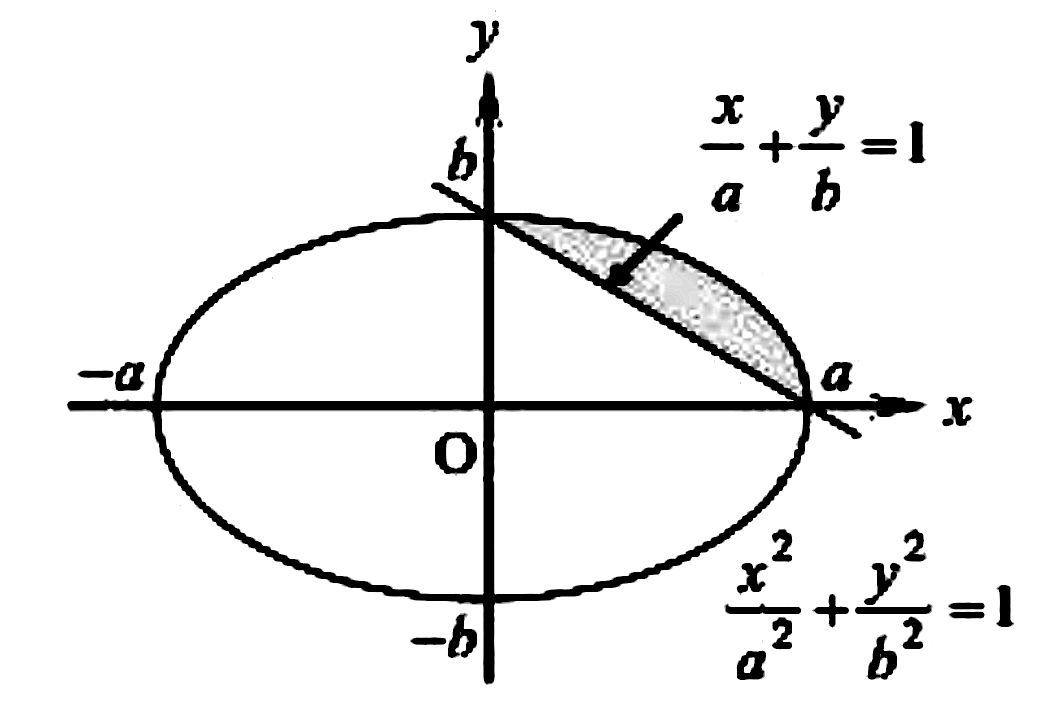
\includegraphics[width=0.35\textwidth]{28-28.4-24.png}
            \end{center}
            \begin{enumerate}
                  \item find $V_x$ and $V_y$. \sol{} \vspace{-0.8cm}
                        \begin{multicols}{2}
                              \begin{flalign*}
                                    V_x & = \pi \int_{0}^{a} \left\{ b^2\left(1 - \frac{x^2}{a^2}\right) - \left[b\left(1 - \dfrac{x}{a}\right)\right]^2\right\} dx & \\
                                        & = b^2 \pi \int_{0}^{a} \left( 1 - \frac{x^2}{a^2} - 1 + \frac{2x}{a} - \frac{x^2}{a^2} \right) dx                         & \\
                                        & = b^2 \pi \int_{0}^{a} \left( \frac{2x}{a} - \frac{2x^2}{a^2} \right) dx                                                  & \\
                                        & = b^2 \pi \left[ \frac{x^2}{a} - \frac{2x^3}{3a^2} \right]_{0}^{a}                                                        & \\
                                        & = b^2 \pi \left( \frac{a^2}{a} - \frac{2a^3}{3a^2} \right) = \frac{\pi ab^2}{3}
                              \end{flalign*}
                              \vfill\null
                              \begin{flalign*}
                                    V_y & = \pi \int_{0}^{b} \left\{ a^2\left(1 - \frac{y^2}{b^2}\right) - \left[a\left(1 - \dfrac{y}{b}\right)\right]^2\right\} dy & \\
                                        & = a^2 \pi \int_{0}^{b} \left( 1 - \frac{y^2}{b^2} - 1 + \frac{2y}{b} - \frac{y^2}{b^2} \right) dy                         & \\
                                        & = a^2 \pi \int_{0}^{b} \left( \frac{2y}{b} - \frac{2y^2}{b^2} \right) dy                                                  & \\
                                        & = a^2 \pi \left[ \frac{y^2}{b} - \frac{2y^3}{3b^2} \right]_{0}^{b}                                                        & \\
                                        & = a^2 \pi \left( \frac{b^2}{b} - \frac{2b^3}{3b^2} \right)  = \frac{\pi a^2b}{3}
                              \end{flalign*}
                              \vfill\null
                        \end{multicols}
                        \vspace{-1cm}

                  \item if $V_x = 2V_y$, find the value of $a:b$. \sol{}
                        \begin{flalign*}
                              \frac{\pi ab^2}{3} & = 2 \cdot \frac{\pi a^2b}{3} & \\
                              b                  & = 2a                         & \\
                              a:b                & = 1:2
                        \end{flalign*}
            \end{enumerate}
\end{enumerate}